Um eine Arbeit mit \LaTeX\ verfassen zu können, benötigen Sie drei Dinge.

\begin{enumerate}
\item Eine \LaTeX-Distribution
  \begin{compactitem}
  \item \TeX\ Live (\url{https://www.tug.org/texlive/}, alle Plattformen, empfohlen)
  \item MiK\TeX\ (\url{http://miktex.org/}, nur Windows)
  \end{compactitem}

\item Einen beliebigen Text-Editor oder einen speziellen \LaTeX-Editor
  \begin{compactitem}
  \item \TeX studio (\url{http://texstudio.sourceforge.net/})
  \item \TeX works (\url{http://www.tug.org/texworks/})
  \item Kile (\url{http://kile.sourceforge.net/})
  \item \TeX nicCenter (\url{http://www.texniccenter.org/})
  \item Texmaker (\url{http://www.xm1math.net/texmaker/})
  \item LEd (\url{http://www.latexeditor.org/})
  \end{compactitem}

\item Einen PDF-Dokumentbetrachter
  \begin{compactitem}
  \item Okular (\url{http://okular.kde.org/})
  \item Evince (\url{https://wiki.gnome.org/Apps/Evince})
  \item Adobe Acrobat (\url{http://get.adobe.com/de/reader/})
  \end{compactitem}
\end{enumerate}


Der \LaTeX-Compiler übersetzt das vom autor geschrieben Manuskript in eine
anzeigbare PDF-Datei. Früher erfolgte die Ausgabe noch im DVI-Format, welches
erst über Zwischenstufen nach PDF umgewandelt werden musst. Dies ist aber
Heutzutage nicht mehr der Fall.

Der Übersetzungsvorgang ist in Abbildung~\ref{fig:intro:compile} dargestellt.
Neben dem Ausgabe-PDF entsteht u.\,a. noch eine Protokolldatei mit der
Dateiendung \texttt{.log}, die Hinweise, Warnungen oder Fehlermeldungen
enthält. Weiterhin entstehen verschiedene temporäre Dateien, die für die
Erstellung von verschiednen Verzeichnissen und für Querverweise im Dokument
notwendig sind. Die Dateien haben verschiedene Endungen. Beispielhaft sind
hier die \texttt{.aux}-Dateien genannt. Der Autor muss sich über diese Dateien
keine Gedanken machen.


\begin{figure}
\centering
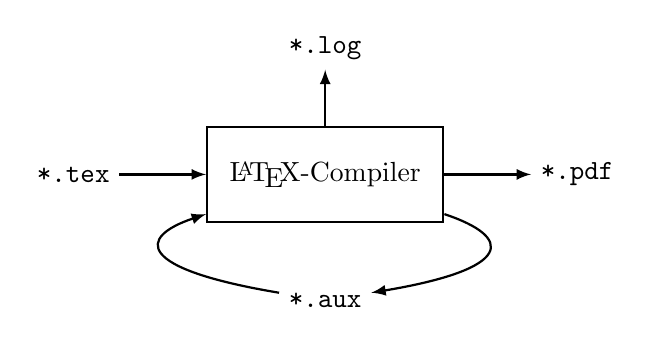
\begin{tikzpicture}[scale=0.8]
\node (latex) at ( 0.0,  0.0) [draw,thick,minimum width=3cm,minimum height=1.2cm] {\LaTeX-Compiler};
\node (tex)   at (-4.0,  0.0) {\texttt{*.tex}};
\node (log)   at ( 0.0,  2.0) {\texttt{*.log}};
\node (aux)   at ( 0.0, -2.0) {\texttt{*.aux}};
\node (pdf)   at ( 4.0,  0.0) {\texttt{*.pdf}};

\draw [-latex,thick] (tex)   -- (latex);
\draw [-latex,thick] (latex) -- (pdf);
\draw [-latex,thick] (latex) -- (log);
\draw [-latex,thick] (latex) .. controls ( 3, -1.0) and ( 3, -1.5) .. (aux);
\draw [-latex,thick] (aux)   .. controls (-3, -1.5) and (-3, -1.0) .. (latex);
\end{tikzpicture}
\caption{Vereinfachter Ablauf des \LaTeX-Übersetzungsvorgangs}
\label{fig:intro:compile}
\end{figure}
